
\section{Low-dimensional and Laplace-correction details}
\label{app:method_details}

\subsection{Flash-SD-KDE in low dimensions}

For completeness we briefly summarize the 1-D SD-KDE arithmetic intensity and
empirical behavior.  With $n_{\text{train}} = k$ and $n_{\text{test}} = k/8$,
there are two steps:
\begin{enumerate}
  \item \textbf{Score + shift:} For each training point we compute
        $\hat s(x_i)$ from all $k$ points and then form
        $x_i^{\mathrm{SD}} = x_i + \tfrac{h^2}{2}\hat s(x_i)$.  This uses
        $O(k^2)$ pairwise kernel interactions.  With the RTX~A6000 hardware
        ratio ($128$ FP32 ALUs, $16$ SFUs per SM) we budget an $\exp$ as
        $8$ flop-equivalents.  The score accumulation requires one $\exp$
        and roughly eight additional arithmetic ops (subtraction, scaling,
        accumulation), yielding $c_1 \approx 16$ flops per
        $(\text{train},\text{train})$ pair.
  \item \textbf{KDE on debiased samples:} We then evaluate a standard Gaussian
        KDE at $k/8$ query points using the $k$ debiased samples, which uses
        $O(k^2/8)$ interactions.  Each pair requires one $\exp$ (8 flops) plus
        about six other operations (difference, square, scaling, accumulation),
        so we take $c_2 \approx 14$ flops per $(\text{train},\text{test})$ pair.
\end{enumerate}
The total work is therefore approximated by
\[
  \text{FLOPs}(k)
  \;\approx\;
  c_1 k^2 + c_2\,k\,(k/8)
  \;\approx\;
  16 k^2 + 14\frac{k^2}{8}
  \;=\;
  17.75\,k^2.
\]
For $k = 32\text{k}$ this is on the order of $2\times 10^{10}$ flops.  When we
fix $n_{\text{test}} = k/8$ we move approximately $5k$ bytes (counting one
read of each train and test point and one write of each output), so the
arithmetic intensity scales as
\[
  I(k)
  =
  \frac{\text{FLOPs}(k)}{\text{Bytes}(k)}
  \;\approx\;
  \frac{17.75\,k^2}{5\,k}
  \approx
  3.55\,k
  \quad \text{flops/byte},
\]
placing realistic problem sizes firmly in the compute-bound regime.

Empirically we sweep $k$ over powers of two from $1024$ to $64\text{k}$, with
$n_{\text{test}} = k/8$, and average over three seeds.  For each
configuration we record scikit-learn Gaussian KDE
time, and SD-KDE Torch time, and Flash-SD-KDE time.  Across the entire range, the Flash-SD-KDE
implementation is consistently faster than scikit-learn, with speedups
growing with $k$; at the largest sizes, Flash-SD-KDE achieves around 2 orders-of-magnitude speedup relative to the sklearn baseline, as shown in Figure~\ref{fig:flash_sd_kde}.

\begin{figure*}[th]
  \centering
  
\includegraphics[width=0.8\linewidth]{figures/runtime_1d_kde_sdkde.pdf}
  \caption{Average runtime (log-scale $y$-axis) of scikit-learn KDE, SD-KDE (Torch), and Flash-SD-KDE across $n_{\text{train}}$ in 1-D; annotations show observed runtimes.}
  \label{fig:flash_sd_kde}
\end{figure*}

%\begin{figure}[th]
%  \centering
%  \includegraphics[width=0.8\linewidth]{figures/emp-sd-kde-%util.pdf}
%  \caption{Estimated GPU utilization (as a percentage of A6000 %FP32 peak)
%           for 1-D SD-KDE implemented in Triton and optimized %Torch,
%           computed from the 1-D flop model and the measured %runtimes.}
%  \label{fig:flash_sd_kde_util}
%\end{figure}

As shown in Figure~\ref{fig:triton_large_util}, we also compare the utilization of Flash-SD-KDE with SD-KDE (Torch) over a range of 1-D problem sizes, using powers of
two for $n_{\text{train}}$ up to $2^{16} \approx 64$ thousand (and
$n_{\text{test}} = n_{\text{train}}/8$).  

\begin{figure*}[th]
  \centering
  
\includegraphics[width=0.8\linewidth]{figures/util_1d_empirical_sdkde.pdf}
  \caption{Utilization of the 1-D Flash-SD-KDE kernel and SD-KDE (Torch) for large
           $n_{\text{train}}$ (powers of two up to $2^{16}$).  Labels show
           the observed runtime for each data size; error bars are omitted
           because a single seed is used per point.}
  \label{fig:triton_large_util}
\end{figure*}


\begin{comment}
\section{Oracle density benchmark for Laplace correction beyond $10^6$}
\label{sec:laplace_corrected}
The results are shown below.
\begin{figure*}[t]
  \centering
  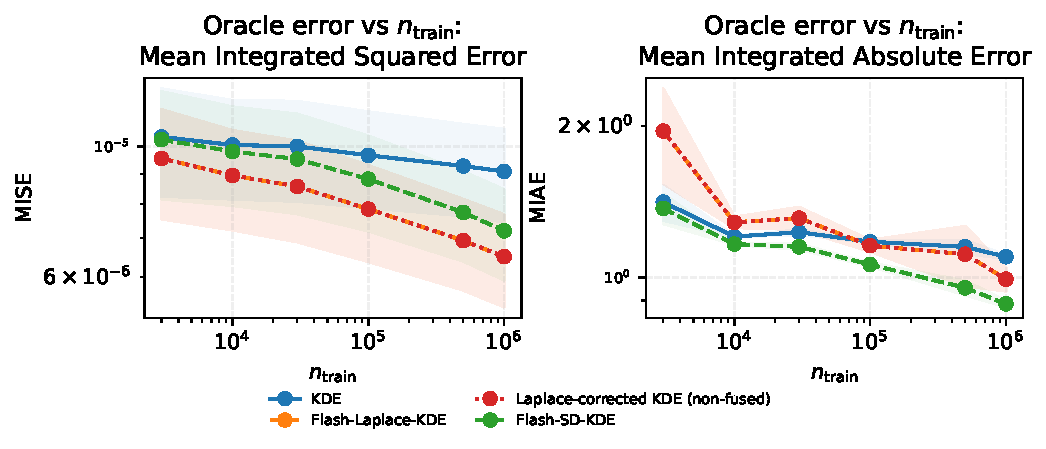
\includegraphics[width=\textwidth]{figures/fig_oracle_error_vs_n_16d.pdf}
  \caption{Oracle error on a 16D mixture-of-Gaussians benchmark.
           We report MISE and MIAE versus $n_{\text{train}}$ for KDE and Flash-Laplace-KDE (fused Laplace correction).}
  \label{fig:e6_fig_oracle_error_vs_n}
\end{figure*}
\end{comment}


% \begin{revadded}
\subsection{Laplace-corrected KDE derivation and 1D benchmarks}
\label{app:laplace_derivation}

% \end{revadded}

% [RED WRAP MOVED LAPLACE FIGURES]
\begin{revadded}
\begin{figure*}[t]
  \centering
  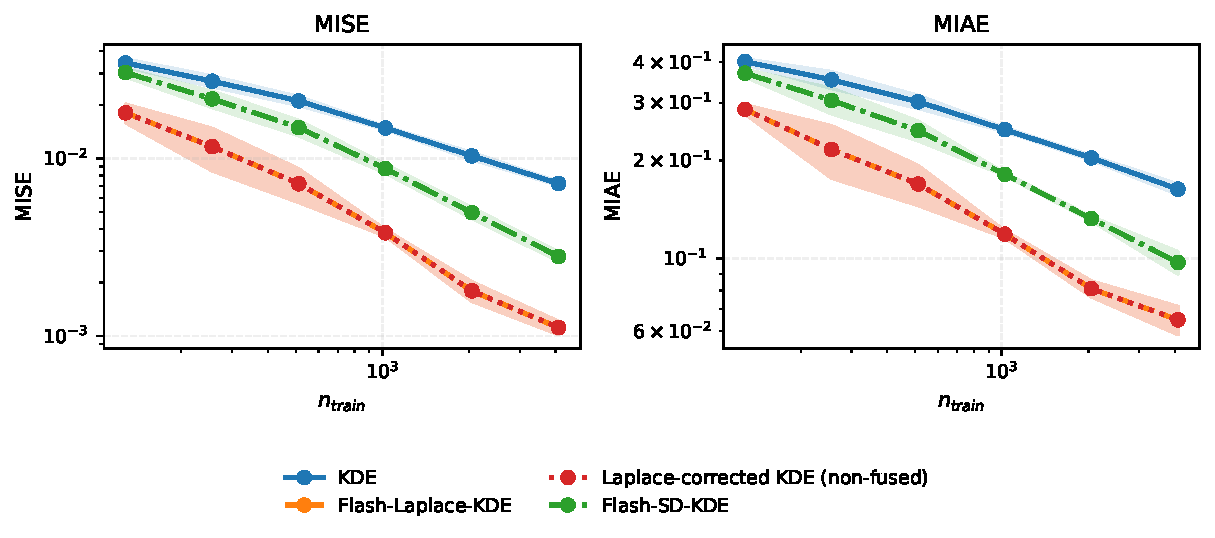
\includegraphics[width=\textwidth]{figures/fig_oracle_error_vs_n_1d.pdf}
  \caption{Oracle error on a 1D mixture-of-Gaussians benchmark.
           We report MISE and MIAE versus $n_{\text{train}}$ for KDE, Flash-Laplace-KDE (fused Laplace correction), non-fused Laplace correction, and Flash-SD-KDE.
           The Laplace-corrected estimators can be slightly negative, so error is computed on the signed density.}
  \label{fig:oracle_error_1d}
\end{figure*}

\begin{figure*}[t]
  \centering
  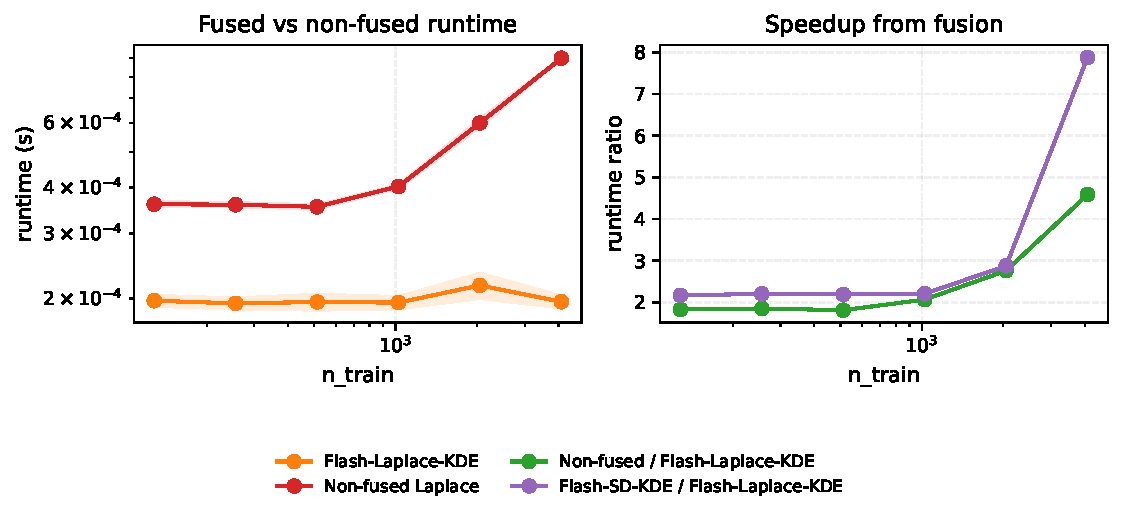
\includegraphics[width=\textwidth]{figures/fig_fused_vs_nonfused_runtime.pdf}
  \caption{Runtime and speedup for Laplace correction in 1D.
           The left panel shows total runtime for the fused Flash-Laplace-KDE kernel and a non-fused implementation.
           The right panel reports speedup ratios, including Flash-SD-KDE relative to Flash-Laplace-KDE for context.}
  \label{fig:laplace_speedup_1d}
\end{figure*}

\end{revadded}
% [END RED WRAP MOVED LAPLACE FIGURES]

% \begin{revadded}
We evaluate Laplace-corrected KDE on a 1D oracle density.
Figure~\ref{fig:oracle_error_1d} compares KDE, Flash-Laplace-KDE (fused Laplace correction), non-fused Laplace correction, and Flash-SD-KDE.
The Laplace-corrected estimators can take small negative values for large $\lVert x - x_i \rVert$.
We therefore compute errors on the signed density, and we report the negative-mass diagnostics separately in the benchmark logs.

Figure~\ref{fig:laplace_speedup_1d} shows the runtime advantage of fusion.
The fused Flash-Laplace-KDE kernel consistently outperforms the non-fused Laplace correction across $n_{\text{train}}$.
For context, the same plot also reports the Flash-SD-KDE to Flash-Laplace-KDE runtime ratio.

As an intuitive explanation of why both methods achieve the same leading bias reduction, we can first view vanilla KDE\footnote{Throughout, we assume that the kernel is Gaussian for simplicity.} as a heat semigroup (kernel) $P_{t} = e^{\frac{t}{2}\Delta}$ with $t = h^2$ applying to the empirical density  function $f_n$ (sampled with replacement) to be
\begin{align*}
    \hat{f} = P_t f_n.
\end{align*}
From the linearity of the heat semigroup, we then have that the expected estimate
\begin{align*}
    \mathbb{E}\left[\hat{f}\right]
    =\mathbb{E}\left[P_t f_n\right]
    =P_t\mathbb{E}\left[ f_n\right]
    =P_tf,
\end{align*}
where $f$ is the true probability density function.

The bias is then, under a smoothness assumption we assume throughout,
\begin{align*}
    \mathbb{E}\left[\hat{f}\right]-f = (P_t-I)f = \frac{t}{2} \Delta f + O(t^2).
\end{align*}

The Laplace kernel deals with this leading term by using an operator $\left(I-\frac{t}{2}\Delta\right)P_t$ instead, making its bias
\begin{align*}
    \mathbb{E}\left[\hat{f}^{\text{LC}}\right]-f = \left[\left(I-\frac{t}{2}\Delta\right)P_t-I\right]f = O(t^2).
\end{align*}

The SD-KDE algorithm approaches this debias task differently by applying a \textbf{non-linear}\footnote{Even when the transportation kernel has a non-linear transportation. The kernel itself is linear.} transportation kernel $T_{\frac{t}{2}\nabla \log f}$ before applying a standard heat kernel $P_t$, making its bias
\begin{align*}
    &\mathbb{E}\left[\hat{f}^{\text{SD-KDE}}\right]-f\\ &= \left[P_tT_{\frac{t}{2}\nabla f}-I\right]f\\
    &=
    \left[P_t\left(f - \frac{t}{2}\nabla \cdot \left(f\nabla \log f\right) + O(t^2)\right)-f\right]\\
    &=
    \left[P_t\left(f - \frac{t}{2}\Delta f + O(t^2)\right)-f\right]\\
    &=
    \left[P_t\left(I - \frac{t}{2}\Delta  \right)-I\right]f+ O(t^2)\\
    &= O(t^2).
\end{align*}
Recall that $t=h^2$, so we have that Laplace KDE and SD-KDE have an $O(h^4)$ bias, while vanilla KDE has an $O(h^2)$ bias.

Note that the analysis above assumes that the SD-KDE has access to the oracle, so the translation kernel is linear. In practice, the score is empirical, making the translation kernel
\begin{align*}
    T_{\frac{t}{2}\nabla \log \left(P_{t'} f_n\right)}
\end{align*}
where $t'=\frac{h^2}{2}$ is the bandwidth for the kernel used for score estimation. Thus, the empirical SD-KDE is
\begin{align*}
    \hat{f}^{\text{Emp SD-KDE}} = T_{\frac{t}{2}\nabla \log \left(P_{t'} f_n\right)} f_n,
\end{align*}
which is no longer linear in $f_n$.
% \end{revadded}
